\section{System Architecture and Design}\label{sec:arch}

\subsection{Architectural overview}

The lab assistant consists of two parts (Figure~\ref{fig:arch}). Two \emph{image-analysis stages} turn a smear image into structured findings: a detector that finds and counts the cells, and a classifier that assigns a type, an uncertainty level and a saliency map to every white cell. The \emph{domain expert} then interprets these findings using hematology knowledge. The expert can be run with a hosted model (GPT-4o inside a tool-using agent) or with the open, fine-tuned Llama model, and it can also be used on its own as a hematology question-answering system.

The pipeline is strictly feed-forward: every stage has a typed input and output, and each stage consumes only the structured output of the previous one, never the raw upstream data. This keeps each stage replaceable --- for example, the detector can be exchanged without retraining the classifier, and the language model can be exchanged without touching the vision stages --- and it produces an inspectable artefact at every step: a box overlay, a label with an uncertainty level, a heatmap, retrieved passages and a tool trace.

\begin{figure}[H]
\centering
\begin{tikzpicture}[
  node distance=0.55cm,
  box/.style={draw=black!55, rounded corners=3pt, align=center, font=\scriptsize, minimum height=1.35cm, text width=2.05cm, fill=white},
  exp/.style={box, fill=blue!6, draw=blue!55!black, text width=2.3cm},
  kb/.style={box, fill=black!4, minimum height=0.8cm, text width=2.2cm},
  arr/.style={-{Stealth[length=2mm]}, thick, draw=black!60}]
\node[box] (img) {Smear image\\(RGB)};
\node[box, right=of img] (s1) {\textbf{Stage 1}\\YOLOv8s\\detector};
\node[box, right=of s1] (s2) {\textbf{Stage 2}\\EfficientNet-B0\\MC-Dropout\\Grad-CAM};
\node[exp, right=of s2] (de) {\textbf{Domain expert}\\GPT-4o ReAct agent\\\emph{or} Llama-3.1-8B\\+ QLoRA};
\node[box, right=of de, fill=green!5, draw=green!40!black] (rep) {\textbf{JSON report}\\interpretation,\\citations, flags,\\tool trace};
\node[kb, above=0.7cm of de, xshift=-1.25cm] (kb) {Textbook vector\\store (1{,}049 chunks)};
\node[kb, above=0.7cm of de, xshift=1.25cm] (tools) {Tools: ranges,\\counts, uncertainty};
\node[box, below=0.8cm of de, fill=orange!8, draw=orange!60!black, minimum height=0.9cm, text width=2.6cm] (rule) {Deterministic\\review rule};
\draw[arr] (img) -- (s1);
\draw[arr] (s1) -- (s2);
\draw[arr] (s2) -- (de);
\draw[arr] (de) -- (rep);
\draw[arr, <->] (kb.south) -- (kb.south |- de.north);
\draw[arr, <->] (tools.south) -- (tools.south |- de.north);
\draw[arr] (de.south) -- (rule.north);
\draw[arr, dashed] (s2.south) |- (rule.west);
\draw[arr] (rule.east) -| (rep.south);
\end{tikzpicture}
\caption{Architecture of the system. Stage~1 returns boxes, classes and confidences; Stage~2 returns, for every white cell, a label, confidence, entropy, uncertainty level and heatmap. The expert queries the knowledge base and tools and writes the report. The dashed arrow shows that the review rule reads the Stage-2 uncertainty directly, independently of the language model.}
\label{fig:arch}
\end{figure}

All runtime parameters --- model paths, thresholds, the number of MC-Dropout passes, chunk size, embedding model, number of retrieved chunks, language model, temperature and agent budget --- are set in a single \code{config.yaml} file. All inference goes through one orchestrator class, \code{BloodSmearPipeline}; the command-line interface and the web backend are thin wrappers around it.

\subsection{Stage 1: cell detection with YOLOv8}\label{sec:stage1}

Given an image $I$, Stage~1 returns a set of boxes $\mathcal{B}(I) = \{(x_1, y_1, x_2, y_2, c, p)_i\}$, where $c \in \{\text{WBC}, \text{RBC}, \text{Platelet}\}$ and $p$ is the detector's confidence. Boxes with $p < 0.50$ are discarded.

The detector is YOLOv8s \cite{jocher2023yolov8}, the ``small'' variant (about 11 million parameters) of a single-stage, anchor-free object detector. It consists of a convolutional backbone, a feature-pyramid neck that fuses information from several scales, and a decoupled head that predicts class scores and box coordinates. The small variant was chosen as a compromise between accuracy and speed on an ordinary laptop CPU. At inference the checkpoint is loaded once and kept in memory, and class names are normalised (\emph{Platelets} and \emph{Platelet} are unified, because source datasets use both). The white-cell boxes are cropped from the image and passed to Stage~2, and the per-class counts are passed to the domain expert.

\subsection{Stage 2: white-cell classification with uncertainty and saliency}\label{sec:stage2}

For each WBC crop, Stage~2 returns
\begin{equation}
  y(\text{crop}) = \big(\hat{c},\ \bar{p}_{(1)},\ H,\ v,\ b,\ \text{Grad-CAM}\big),
\end{equation}
the predicted class, its mean probability (confidence), the predictive entropy, the mean variance across passes, an uncertainty level $b \in \{\text{LOW}, \text{MEDIUM}, \text{HIGH}\}$, and a saliency overlay.

\paragraph{Classifier.} The backbone is EfficientNet-B0 \cite{tan2019efficientnet} from the \code{timm} library, pre-trained on ImageNet. Its 1{,}000-class head is replaced by a small multilayer head: Linear(1280$\to$1024) -- ReLU -- Dropout(0.3) -- Linear(1024$\to$512) -- ReLU -- Dropout(0.3) -- Linear(512$\to$8). The two dropout layers are what makes MC-Dropout possible.

\paragraph{Monte Carlo Dropout.} At prediction time the network is put into evaluation mode and then only its \code{nn.Dropout} modules are switched back to training mode; batch-normalisation layers stay in evaluation mode so that their statistics do not drift. Each crop is passed through the network $T = 20$ times, giving a $T \times C$ matrix of class probabilities. The mean $\bar{p}$ over the passes is the prediction, $\bar{p}_{(1)}$ is its largest entry, $H = -\sum_c \bar{p}_c \log \bar{p}_c$ is the predictive entropy, and $v$ is the per-class variance across passes averaged over the classes. The uncertainty level is then
\begin{equation}
b = \begin{cases}
\text{LOW} & \text{if } \bar{p}_{(1)} \ge 0.85 \text{ and } H < 0.3,\\
\text{MEDIUM} & \text{else if } \bar{p}_{(1)} \ge 0.65 \text{ and } H < 0.6,\\
\text{HIGH} & \text{otherwise.}
\end{cases}
\end{equation}
A HIGH cell is marked as \emph{flagged}. The thresholds are set in the configuration file; they were chosen by hand and have not been calibrated against error rates.

\paragraph{Grad-CAM.} For each crop, the predicted class score is back-propagated to the network's final convolutional layer (\code{conv\_head}), the Grad-CAM map (Equation~2) is up-sampled to $224 \times 224$ and blended over the crop with an opacity of 0.45. The resulting image is returned with the prediction and shown in the user interface.

\subsection{Stage 3: domain-expert reasoning --- knowledge base and retrieval (RAG)}\label{sec:kb}

The 1{,}049 textbook chunks (Section~\ref{sec:corpus}) are embedded with the sentence-transformer \code{all-MiniLM-L6-v2} \cite{reimers2019,wang2020minilm}, a six-layer model that maps a text to a 384-dimensional vector and runs quickly on a CPU. The vectors are stored in a persistent ChromaDB collection \cite{chroma} with cosine distance, so the index is built once and re-used; it is rebuilt automatically if the number of stored chunks does not match the corpus. For a query, the query text is embedded with the same model and the five most similar chunks are returned with their source and chunk index. The complete pipeline is shown in Figure~\ref{fig:rag}. An optional web-search extension, restricted to an allow-list of medical domains (e.g.\ NCBI, MedlinePlus, WHO), exists but is disabled in all experiments for reproducibility.

\begin{figure}[H]
\centering
\begin{tikzpicture}[
  node distance=0.5cm,
  st/.style={draw=black!55, rounded corners=3pt, align=center, font=\scriptsize, minimum height=1.0cm, text width=2.0cm, fill=white},
  db/.style={st, fill=black!4},
  arr/.style={-{Stealth[length=2mm]}, thick, draw=black!60}]
% offline row
\node[font=\scriptsize\bfseries, anchor=west] (off) at (-1.2,1.35) {Offline (once)};
\node[st] (pdf) at (0,0) {2 textbook PDFs\\(541 pages)};
\node[st, right=of pdf] (ext) {Text extraction\\(\code{pypdf})};
\node[st, right=of ext] (chk) {Chunking\\200 words,\\40 overlap};
\node[st, right=of chk] (emb) {Embedding\\MiniLM-L6-v2\\(384-d)};
\node[db, right=of emb] (vdb) {ChromaDB\\1{,}049 vectors\\(cosine)};
% online row
\node[font=\scriptsize\bfseries, anchor=west] (on) at (-1.2,-1.55) {At question time};
\node[st, below=1.9cm of pdf] (q) {Query from\\the agent};
\node[st, right=of q] (qe) {Embed query\\(same model)};
\node[st, right=of qe] (top) {Top-5 nearest\\chunks};
\node[st, right=of top] (ref) {Numbered as\\{[}Reference N{]}};
\node[st, right=of ref, fill=blue!6, draw=blue!55!black] (llm) {LLM answer\\with citations};
\draw[arr] (pdf) -- (ext); \draw[arr] (ext) -- (chk); \draw[arr] (chk) -- (emb); \draw[arr] (emb) -- (vdb);
\draw[arr] (q) -- (qe); \draw[arr] (qe) -- (top); \draw[arr] (top) -- (ref); \draw[arr] (ref) -- (llm);
\draw[arr, dashed] (vdb.south) |- ($(top.north)+(0,0.45)$) -- (top.north);
\end{tikzpicture}
\caption{The retrieval-augmented generation (RAG) pipeline. The knowledge base is built once; at question time the agent's query is embedded with the same model and the five most similar chunks are returned, numbered so that the model can cite them.}
\label{fig:rag}
\end{figure}

\subsection{Stage 3, backend A: GPT-4o with tools (ReAct agent)}\label{sec:agent}

The main runtime expert is GPT-4o \cite{openai2024gpt4o}, called at temperature 0.1 through the OpenAI API. GPT-4o was chosen because it follows structured-output and tool-calling instructions reliably and needs no local GPU. The model is wrapped in a LangGraph ReAct agent \cite{yao2023react,langgraph} with the five tools listed in Table~\ref{tab:tools}.

\begin{table}[H]
\centering
\caption{Tools available to the domain-expert agent.}
\label{tab:tools}
\small
\begin{tabularx}{\textwidth}{>{\raggedright\arraybackslash}p{5.6cm} X}
\toprule
\textbf{Tool} & \textbf{Purpose} \\
\midrule
\code{query\_knowledge\_base} & Takes a search query; retrieves the top-5 textbook chunks and numbers them as \code{[Reference N]}. \\
\code{lookup\_lab\_reference\_ranges} & Takes a parameter name; returns a typical adult reference range (e.g.\ monocytes 2--8\,\% of WBC). \\
\code{interpret\_differential} & Takes the differential as JSON; compares each class percentage with its reference range and reports LOW/HIGH/normal. \\
\code{get\_uncertainty\_summary} & Returns the Stage-2 MC-Dropout statistics (number of flagged cells). \\
\code{get\_detection\_counts} & Returns the Stage-1 cell counts for the field of view. \\
\bottomrule
\end{tabularx}
\end{table}

The system prompt tells the agent to call the knowledge base one to three times to ground its claims, to look up reference ranges before calling a value abnormal, to review the uncertainty summary before making confident statements, to cite evidence as \code{[Reference N]}, to give differential rather than definitive diagnoses, and to remember that the counts are per microscope field and must not be converted into clinical concentrations. The final message must be a JSON object with the fields \code{clinical\_interpretation}, \code{key\_findings}, \code{differential\_diagnoses}, \code{recommendations}, \code{safety\_flags}, \code{requires\_expert\_review} and \code{confidence\_assessment}. The number of reasoning steps is bounded through LangGraph's recursion limit (derived from a configured maximum of six iterations), and every tool call and tool result is returned to the user as the \emph{agent trace}.

A simpler \emph{linear} mode is also available: one retrieval followed by one LLM call with the retrieved chunks in the prompt. In linear mode the code checks that the cited reference numbers actually exist among the retrieved chunks, and it adds an \code{INSUFFICIENT\_EVIDENCE} flag if no valid citation or no differential diagnosis is returned.

The language-model client talks to any OpenAI-compatible endpoint. Replacing GPT-4o by a self-hosted model therefore only requires changing the model name in \code{config.yaml} and the \code{OPENAI\_BASE\_URL} environment variable.

\subsection{Stage 3, backend B: a fine-tuned open-weight model}\label{sec:ft}

The second form of the expert is an open-weight model adapted to the domain, which can run on local hardware. The base model is \textbf{Llama-3.1-8B-Instruct} \cite{grattafiori2024llama3}, loaded in 4-bit precision, and it is adapted with \textbf{QLoRA} \cite{dettmers2023qlora}: LoRA adapters of rank $r=16$ ($\alpha = 32$, no dropout) are attached to all attention and feed-forward projections (\code{q, k, v, o, gate, up, down}), which adds 41.9 million trainable parameters --- 0.52\,\% of the model's 8.07 billion. The adapter is trained on the 1{,}890 training pairs (Section~\ref{sec:qa-data}), so the model learns to answer hematology questions in the form of the textbook-grounded answers. The resulting adapter (about 42 million parameters, roughly 84\,MB in 16-bit precision) can be served, for example with vLLM, behind an OpenAI-compatible endpoint and selected in the configuration without changing any other part of the system. Training details are given in Section~\ref{sec:ft-train}.

It is important to note what the training examples contain: a system prompt, a question and an answer --- but \emph{not} the textbook passage. The fine-tuned model therefore learns to answer from its weights, not to read and cite a retrieved passage. This design choice turns out to matter for how its citations should be interpreted (Section~\ref{sec:res-de}).

\subsection{Safety logic: the expert-review rule}\label{sec:safety}

Two design principles guide the safety behaviour. First, safety-relevant information is always passed forward and shown: every detection carries its confidence, every classified cell its uncertainty level and heatmap, every interpretation its tool trace. Second, the decision whether a human must review the case is not left to the language model alone. The flag \code{requires\_expert\_review} starts from the model's own judgement, but deterministic code \emph{forces it to true} whenever at least one Stage-2 cell is flagged as HIGH uncertainty, and adds a \code{HIGH\_UNCERTAINTY} safety flag. In linear mode, missing citations also force the flag. A second rule, added after the case study in Section~\ref{sec:case} revealed the gap, checks the \emph{number} of classified white cells: if it is below a configurable minimum (\code{llm.safety.min\_wbc\_for\_differential}, default 100, following the convention of counting at least 100 cells for a differential \cite{clsi2007h20}), an \code{INSUFFICIENT\_CELL\_COUNT} flag is added and review is forced. Both reasoners are also told the cell count and instructed not to interpret percentages when it is insufficient. The rules are implemented in \code{src/utils/safety\_rules.py} and applied by the pipeline after either reasoner has answered, so they hold in both modes. The code can only raise the flag, never lower it. Stage-1 detection confidence does not influence the flag.

\subsection{Software implementation and user interface}\label{sec:software}

The system is implemented as a Python library (\code{src/}) with a FastAPI backend (\code{backend/}) and a React + TypeScript web interface (\code{frontend/}). The backend exposes \code{GET /api/health}, \code{GET /api/samples} and \code{POST /api/analyze}; the latter accepts an image (and optionally a JSON object with CBC laboratory values) and returns the full JSON result. The pipeline is loaded lazily on the first request. The interface shows five panels: the detection overlay with cell counts, the WBC differential with per-cell uncertainty, the Grad-CAM heatmaps, the expert's interpretation with citations and safety flags, and the agent trace (Figures~\ref{fig:ui-a} and~\ref{fig:ui-b}). Thirty-four automated \code{pytest} tests cover configuration loading, batch logic, parsing of model output, retrieval fall-backs, the uncertainty schema, the CBC analyser, the minimum-cell rule and the prompts given to the reasoners. The 29 tests that do not require PyTorch and the trained model files were run for this thesis and all passed; the remaining five load the models and must be run in the project's full environment. The training notebooks for all three models are included and can be run on Google Colab.

The optional CBC input deserves a remark. A small module converts laboratory values (WBC, hemoglobin, MCV, platelets, etc.) into findings such as \emph{leukocytosis} or \emph{microcytosis} with a mild/moderate/severe grade. The findings are added to the prompt of both reasoners (in the agent's input message, and in linear mode also to the retrieval query), together with an instruction to reconcile them with the image findings. The web interface does not yet have a CBC input field, so CBC values can currently only be supplied through the API. Because no experiment in this thesis uses CBC values, this feature is presented as an implemented extension, not as an evaluated result.

\begin{figure}[H]
\centering
\begin{subfigure}{\textwidth}\centering
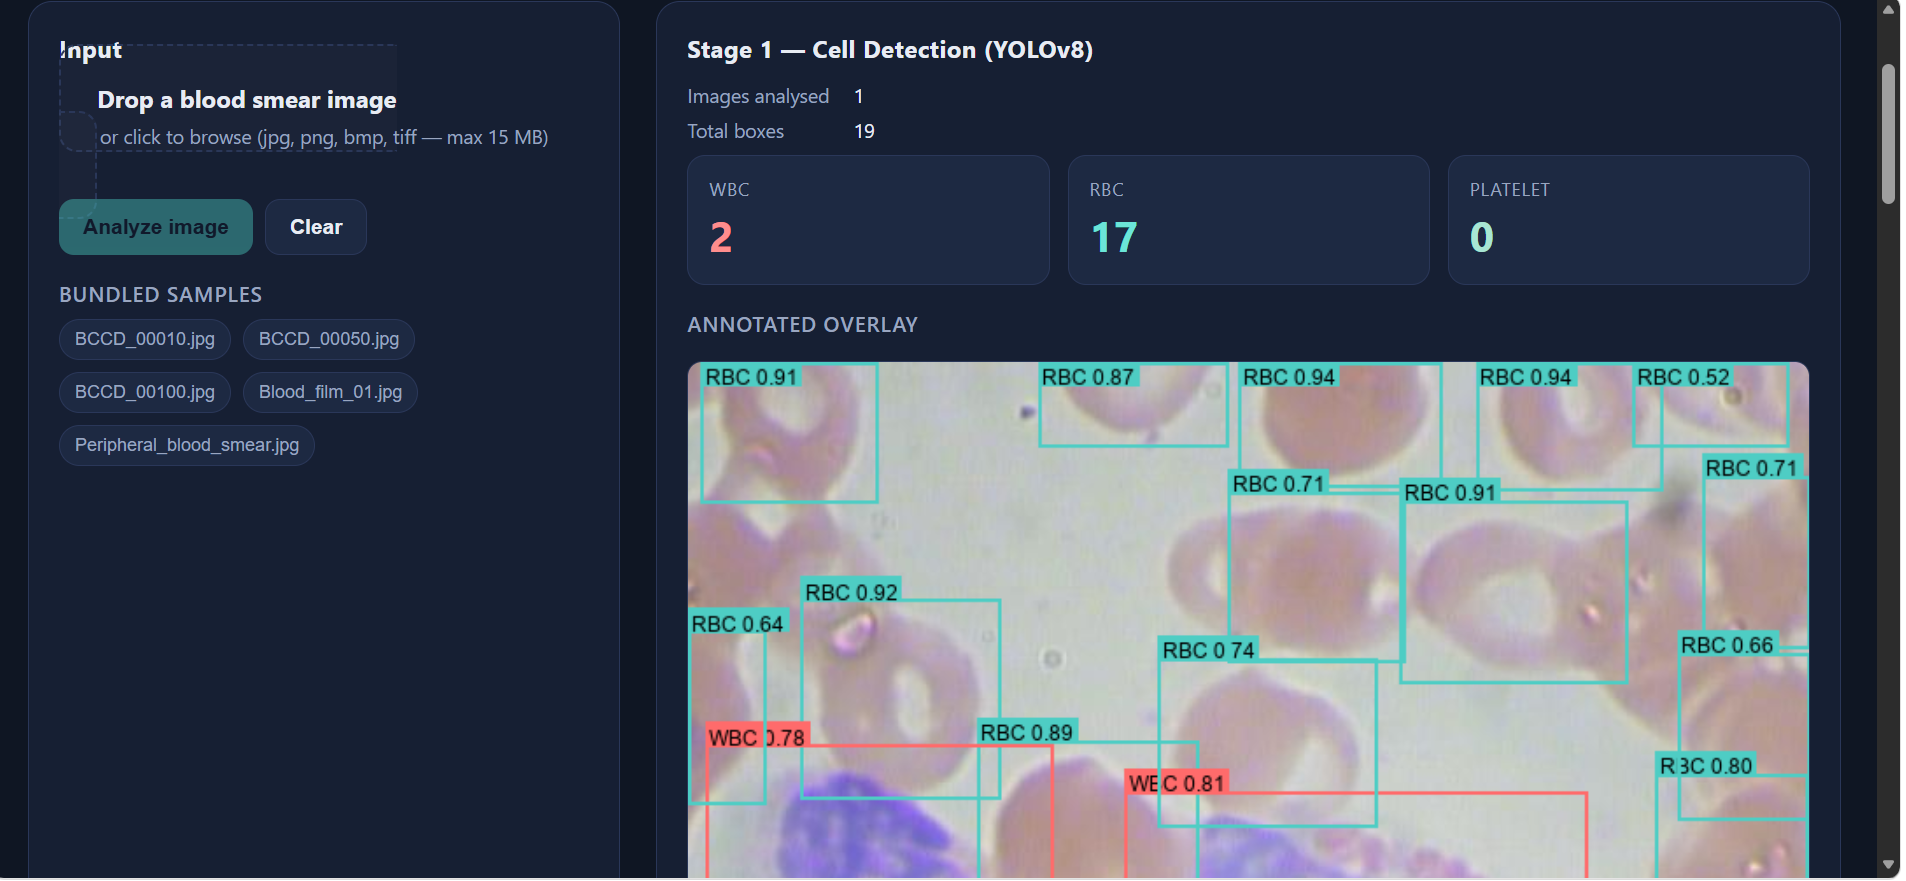
\includegraphics[width=0.95\textwidth]{figures/01_detection.png}
\caption{Detection panel: boxes and per-class counts.}
\end{subfigure}\\[6pt]
\begin{subfigure}{\textwidth}\centering
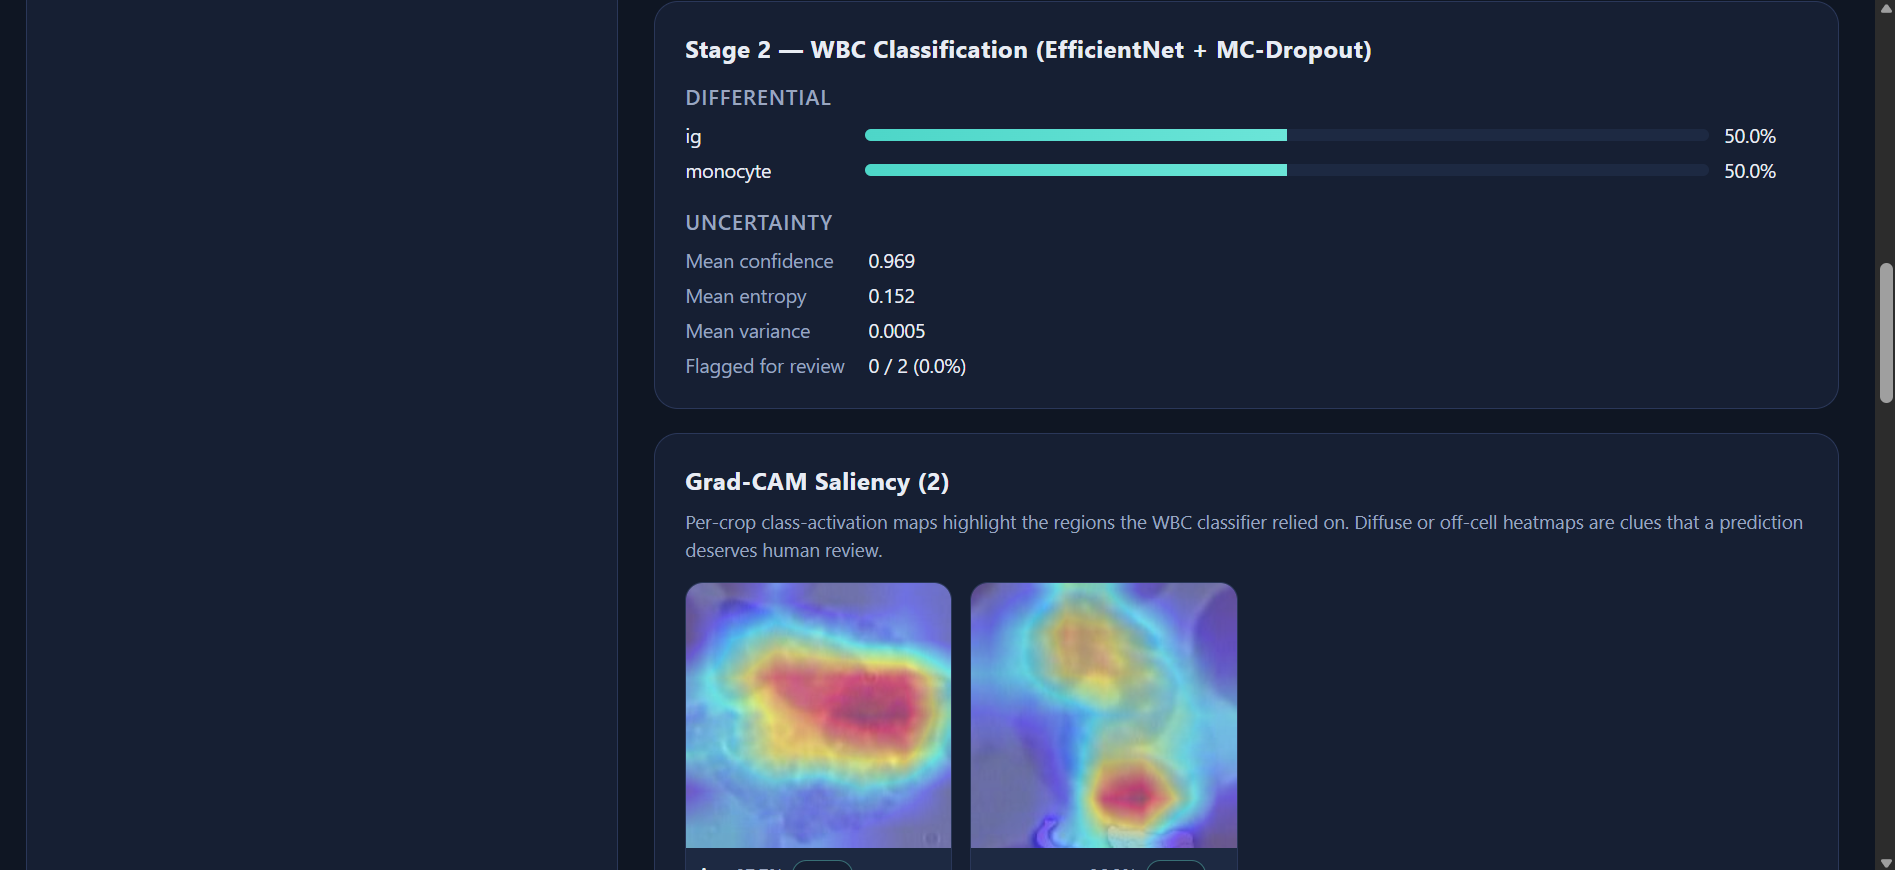
\includegraphics[width=0.95\textwidth]{figures/02_classification_gradcam.png}
\caption{WBC differential, per-cell uncertainty and Grad-CAM heatmaps.}
\end{subfigure}
\caption{Web interface: image-analysis stages, on sample image BCCD\_00100.}
\label{fig:ui-a}
\end{figure}

\begin{figure}[H]
\centering
\begin{subfigure}{\textwidth}\centering
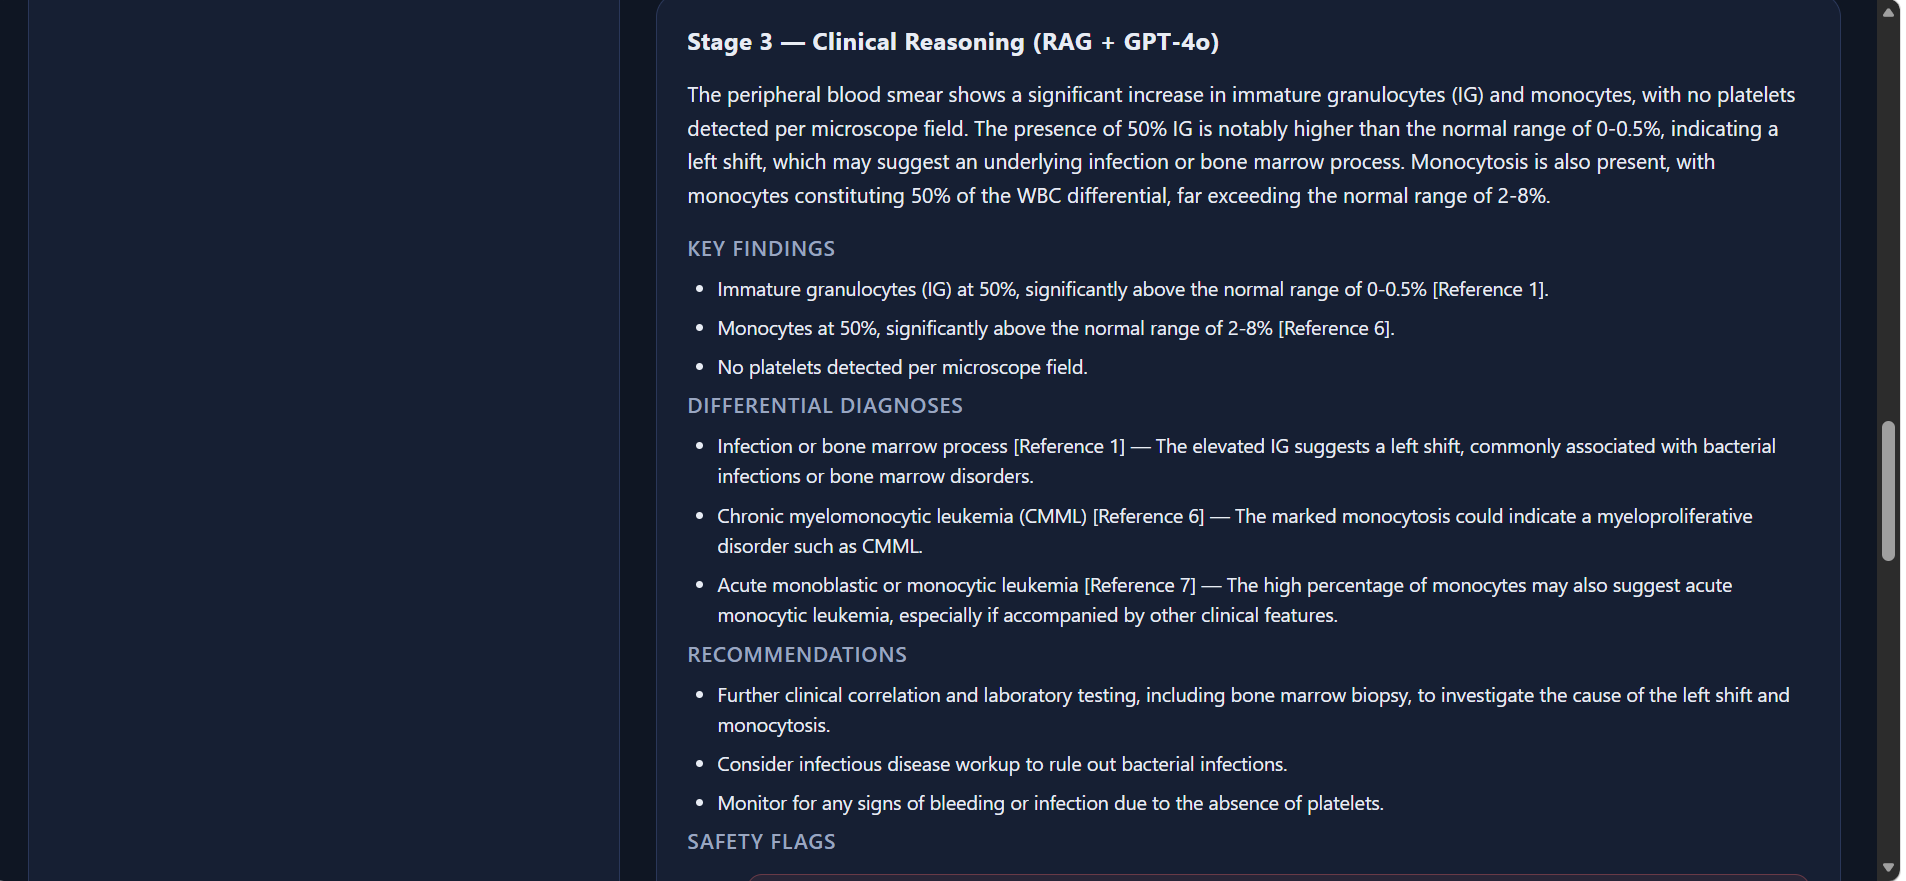
\includegraphics[width=0.95\textwidth]{figures/03_reasoning.png}
\caption{The expert's interpretation with citations and safety flags.}
\end{subfigure}\\[6pt]
\begin{subfigure}{\textwidth}\centering
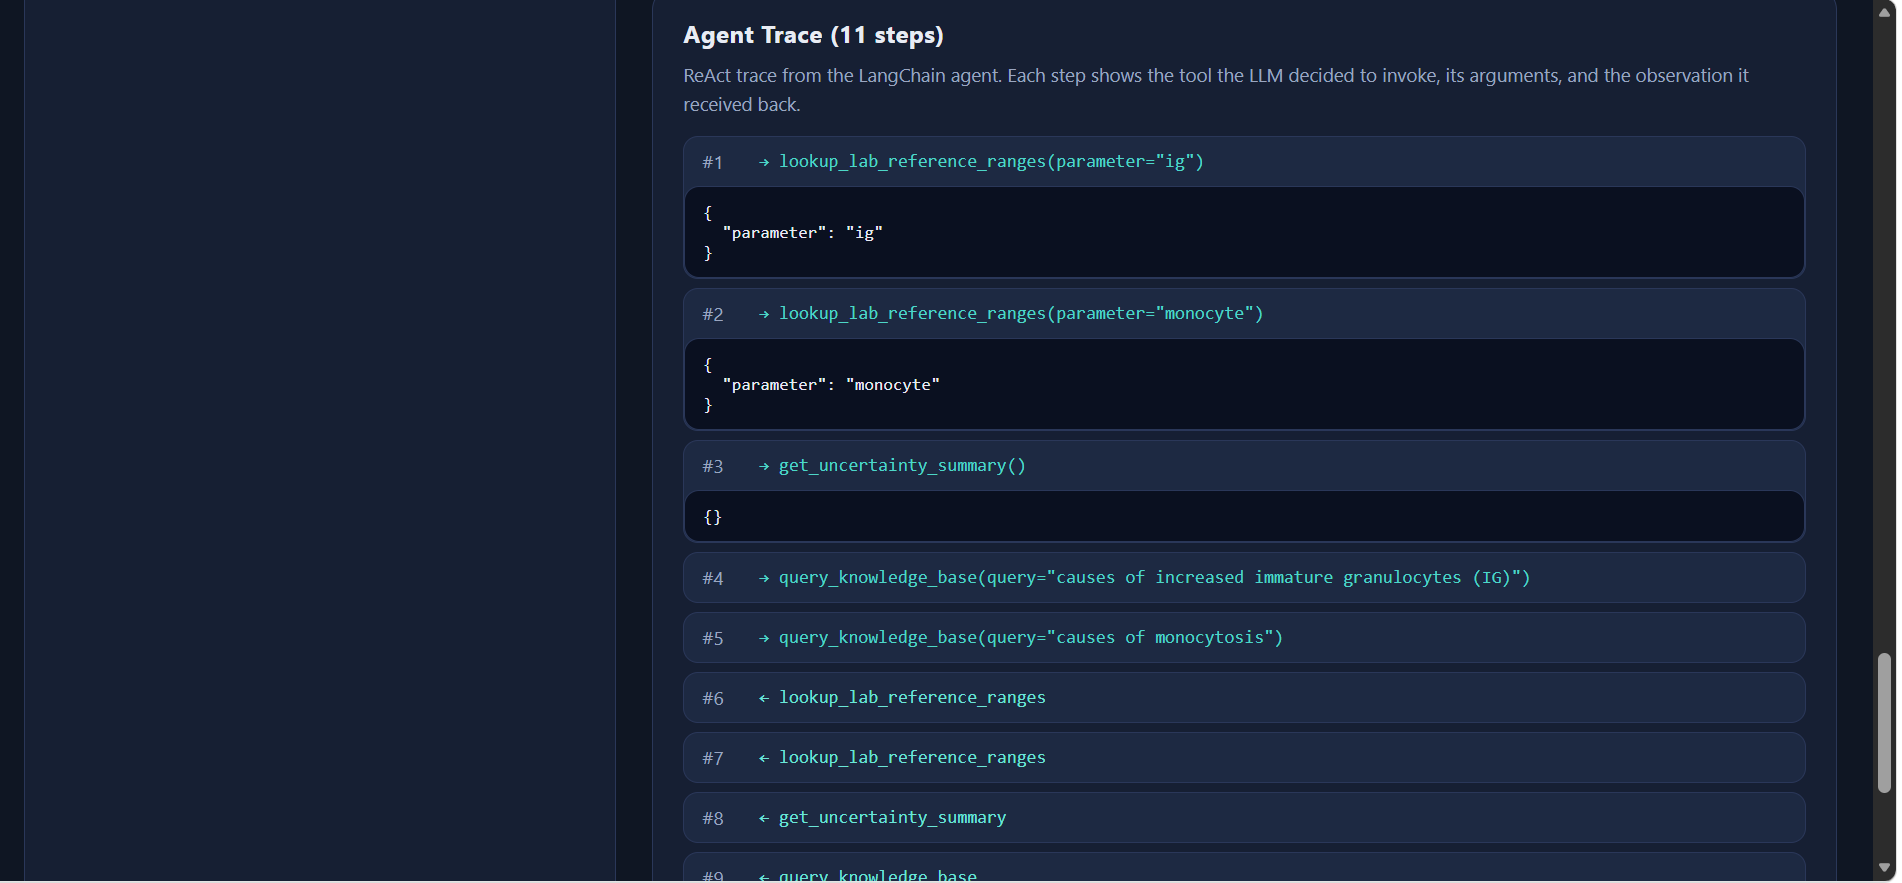
\includegraphics[width=0.95\textwidth]{figures/04_agent_trace.png}
\caption{Agent trace: the sequence of tool calls and results.}
\end{subfigure}
\caption{Web interface: domain-expert output.}
\label{fig:ui-b}
\end{figure}

\clearpage
